\documentclass[11pt, notitlepage]{article}
\usepackage[margin=1in]{geometry}  % Custom margins
\usepackage{tabularx}  % Author block table magic
\usepackage{multicol}
\usepackage{graphicx}
\usepackage[table]{xcolor}\usepackage{titlesec}

% Set space between columns
\setlength\columnsep{25pt}

% Set section titles
\setcounter{tocdepth}{5}
\setcounter{secnumdepth}{5}

% Create figure counter and command to increment and show at the same time
\newcounter{figure_counter}
\newcommand\figuretitle{\addtocounter{figure_counter}{1}Figure \arabic{figure_counter}: }

% Hide page numbers
\pagenumbering{gobble}

% Set path for images
\graphicspath{ {./images/} }


% Begin title region.
\title{\textbf{An Explainable Machine Learning Approach to Antenna Design}}
\author{Tyler Carr \\ carrt12@my.erau.edu \\ Embry-Riddle Aeronautical University \\ Daytona Beach, FL}
\date{}

\begin{document}
\maketitle


\begin{multicols}{2}

\section*{Abstract}
Antenna design process require extensive simulations tasks that are resource and time intensive, and are prone to interruptions. Furthermore, design equations are only available for predefined limited set of antenna geometries. By applying a machine learning algorithm to data that has already been generated from simulations of an antenna, performance metrics can be predicted significantly quicker than running full simulations. Insights about which geometric parameter had the most significant impact on the prediction can be drawn from the model and included in the output. Additionally, the model can be reversed so that for a particular form of antenna, an optimal geometry can be produced that will result in a specified performance. 


\section{Introduction}
Antenna designs require simulation in order to determine the performance of the antenna. Ansys High Frequency Simulation Software (HFSS) is an electromagnetic simulation software which is used to design and simulate the frequency of antennas. When designing the antenna, details such as dimensions of the antenna geometry, materials used for the antenna, and frequency are specified~\cite{Maxworth_2022}. Simulations are then run.


\subsection{Input Data}
The input to the simulation is a table that consists of every permutation of the varying values of each dimension, with each dimension having a set range and a certain value that it is incrementing by. This is also associated with a frequency value. Each permutation is associated with a particular S11 value. S11 value are used as a measure of performance. An S11 value, also known as the reflection coefficient, represents the amount of power reflected from the antenna. An example of an S11 value is 0dB, which would mean that all of the power is being reflected from the antenna, meaning that there is no radiation. Ideally, this value should be below -10dB~\cite{Bevelacqua_2015}. 


\subsection{Simulation Issues}
The main issue with running simulations in HFSS is the amount of time that it takes. The matrix operations that are required to run many iterations of simulations to analyze loss can take multiple days to complete~\cite{john_antenna_2009}. Depending on how the simulation is set up, this process could be impacted by power outages or software bugs, resulting in a loss of data and requiring manual intervention to re-run the simulation. 

HFSS works by specifying a range of dimensions and outputting performance metrics, such as S11 values. This is insightful, but there is a degree of trial and error involved in finding an optimal antenna geometry. One would start by specifying what they would think would be the ideal antenna geometry using their own intuition. Based on the results from an initial simulation run, geometry values would be adjusted in an attempt to optimize the geometry.

By using a machine learning algorithm to do the bulk of the investigative work, the amount of simulation iterations that need to be run can be significantly reduced. The algorithm can then be used to fill in the missing gaps between the reduced data with estimates, making it easier to narrow down to a specific area of interest. 

\subsection{Reversing the Problem}
After training a machine learning model on the permutation data, predictions can be searched by specifying the S11 value of the desired performance and a range of frequency values. Antenna geometries that match the search are returned, which saves significant time that would be required to set up and perform additional simulations.  


\section{Related Work}
TODO FINISH ME


\section{Methodology}
In order to determine the optimal antenna geometry, a machine learning algorithm was employed. This algorithm is trained on the input data, which is the table where each row represents a permutation of geometry dimensions, frequency, and associated S11 value. The X values are the features, which are the geometry dimensions and frequency. The y values are the targets, or the dependent variables. These are the S11 values. After the algorithm is trained, the 

TODO INSERT WHAT TYPE OF ALGORITHM USED AND WHY

TODO  FINISH ME:

- For the development of the algorithm, a Grounded CPW Leaky Wave Antenna was used. This is a new antenna design that was in development by a student which needed refinement.

- Data points with S11 values that are greater than zero are ignored. This should never happen in a real scenario, and means an error occurred with the calculation.

- In order to determine if a S11 value was predicted accurately, a tolerance was utilized. An exact prediction of an S11 value down to multiple decimal points of precision is very unlikely, so this tolerance allows allows for some flexibility. The tolerance is the error that we allow the value to contain, and we consider the prediction accurate if it is within the range above or below the true value. The tolerance is important for an accurate model, and ideally this value should be less than or equal to one.

- Previously, small increments of data would have to be simulated and manually inspected for performance, which takes a lot of time to perform. Training the machine learning model on data with larger increments allows for a shorter simulation time, since the model will fill in the gaps with predictions. It also aids in providing a better guess of an optimal algorithm for a particular performance, helping optimize the antenna faster. 

\begin{center}
  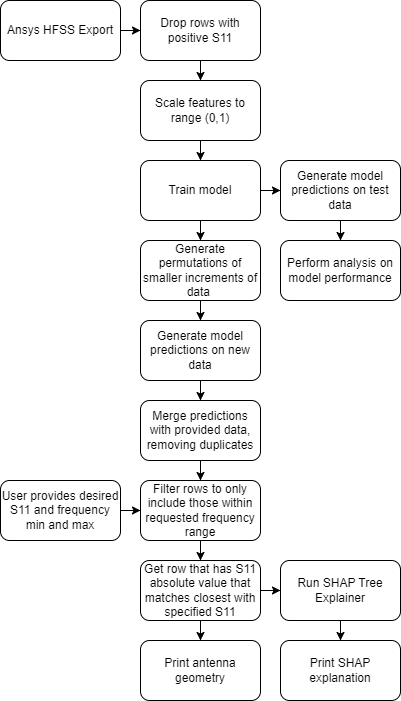
\includegraphics[width=.5\textwidth]{methodology}
  \figuretitle Flow of data through the system
\end{center}

- Insert graph of accuracy here 


\section{Approach}
Blah


\section{Discussion}
Blah


\section{Conclusion}
Blah


\bibliographystyle{unsrt}
\bibliography{refs}


\end{multicols}


\end{document}